\newpage
\section{Process Perspective}

%A description and illustration of:


%  - How do you interact as developers?
%  - How is the team organized?
%  - A complete description of stages and tools included in the CI/CD chains.
%    -  That is, including deployment and release of your systems.
%  - Organization of your repositor(ies).
%    - That is, either the structure of of mono-repository or organization of artifacts across repositories.
%    - In essence, it has to be be clear what is stored where and why.
%  - Applied branching strategy.
%  - Applied development process and tools supporting it
%    - For example, how did you use issues, Kanban boards, etc. to organize open tasks
%  - How do you monitor your systems and what precisely do you monitor?
%  - What do you log in your systems and how do you aggregate logs?
%  - Brief results of the security assessment.
%  - Applied strategy for scaling and load balancing.
%  - In case you have used AI-assistants for writing code during your project or to write the report:
%    - Explain which system(s) you used during the project.
%    - Reflect how it supported/hindered your process.


%In essence it has to be clear how code or other artifacts come from idea into the running system and everything that happens on the way.

\subsection{Teamwork}
\subsubsection{Team agreement}
Within the period where the project was worked on, the team formed some rules and guidelines based on some of the points presented in the "Three Ways" to characterize DevOps from "The DevOps Handbook"\footnote{https://www.oreilly.com/library/view/the-devops-handbook/9781457191381/}: Flow, Feedback and Continual Learning/Experimentation . This was to enhance efficiency and ensure transparency within the group.

\noindent To ensure flow, we did the following:
\begin{itemize}
    \item Mostly through communication on discord, but also through the use of Github projects, we made work visible and transparent for each other. % make work visible
    \item Utilized a small batch strategy, where single features are developed, pushed, and deployed at a time. % reduce batch sizes
    \item By utilizing continuous integration and deployment we limited the amount of intermediary steps, which had to be manually executed. % reduze handoffs
    \item By being aware of what limitations our architecture and processes bring. Early on we realized that our CI/CD tools making a new database at each deployment was not a good idea, and moved to a managed database. %evaluate constraints 
    \item We tried to reduce working on tasks which did not grant any value to the customer by minimizing dead code, feature switching, and manual work. %eliminate hardships
\end{itemize}

\noindent To ensure feedback, we did the following:
\begin{itemize}
    \item We used logs, monitoring, and testing to automate quality checking and see problems as they occurred, and communicated them to the team, if they could not be solved immediately. % see problems as they occur
\end{itemize}

\noindent To ensure continual learning and experimentation, we did the following:
\begin{itemize}
    \item We kept an open discussion about what we could improve and automatize in our work such as when we automatized releases.
    \item Ensuring a learning culture by sharing knowledge at weekly meetings and being open about personal strengths and weaknesses. 
\end{itemize}

\subsubsection{Working schedule}
The team's interaction has been physical at ITU and online through Discord. The primary working day was Tuesday after the exercise session. First, we solved the exercises together and then implemented the feature in our system. If there were leftover work, we would split into subgroups, as different schedules made it difficult to meet physically more than once a week. Since most of the features and tools were new to the group, the overall focus was on implementing and correctly using them. This led us to use pair programming, where one team member shared his screen, and others provided input. The other team members would write code individually if the work were trivial. This was to speed up the process, especially when working with something we did not initially understand.

We incorporated retrospectives from Scrum every Tuesday before we began working on the following week's tasks. This means that we discussed what had been implemented since last Tuesday to share our individual knowledge with the group.

\subsection{CI/CD}
We used GitHub Actions to implement our CI/CD. Our CI/CD consists of test, deploy, release, and code quality analyzer. When a developer pushes his commits, GitHub Actions will run the following steps:

\subsubsection{Code quality analyzer}
SonarCloud was used as a code quality analyzer to analyze the technical debt of the code base. Our repository contains badges about technical debt, security, vulnerabilities, and bugs based on the latest commit to SonarCloud. We also used the C\# linting tool \textit{code-cracker}, but this was only used when building on developer machines and not a part of the workflow. Furthermore, we have used Snyk to scan the project, which is not part of the workflow either.

\subsubsection{Build and Test}
We have different tests as a quality gate before deploying and releasing. We have refactored and expanded the Python tests from the exercises. The system is built on the workflow server via Docker-Compose. First, we have a smoke test to verify that essential elements of the application are functional. Second, we use integration tests to test the API. Last, we use Selenium for end-to-end tests. The Python tests interact with the system via HTTP.

\subsubsection{Deployment}
If the tests are successful, the push will be deployed. First the new image for the application server is pushed to Docker Hub. Then, via ssh, a script is executed on the deployed manager node which pulls the image and redeploys the system.

%We have omitted code reviews and branches to push new code faster. This is to prevent potential dead, local code that is not being used since we value that our code should be used when it works.

\subsubsection{Release}
After deploying the application, we use Versionize and Husky for automatic releases on GitHub. Husky is a linter for commit messages, which checks that a commit message contains the right format. Versionize increments the release version when desired. If the deploy was successful, and the commit message increments the release tag, then our pipeline creates a new release.

\subsection{Repository organization}
We use a mono repository for our source code. We have a trunk-based development, meaning developers push directly to the main branch. If the commits pass the GitHub Workflow, then they will be released. We omitted code reviews because we thought it took too much time to do them. Initially, we considered using it for knowledge sharing. However, since we used pair programming, we already had a way of knowledge sharing. This way we could release new code fast.

\subsection{Development Process}
To keep track of issues and tasks which need to be done, we have experimented with using GitHub Projects as a Kanban board. We have not used this feature rigorously since the course structure already provided some structure of what needed to be done and when. The primary usage has been when we split our group into many parts (individual work) and needed to keep track of it. Mostly development has happened in group work, either all together or split into two groups. Since our project and group size are relatively small, it is still possible to hold developers accountable by reviewing the commit history. However, a more rigorous use of the Kanban board would have made it possible to measure implementation progress retroactively. 

\subsection{Monitoring \& Logging}
During the lifetime of a system, it is rare for everything to work smoothly and without any problems. System components will break down. The system will crash in production, server response times will grind to a halt, and so on. To (1) be able to estimate when the system is not operating within the expected limits and (2) be able to track down the source of this disturbance, it is necessary to have monitoring and logging setup in the project.

Our monitoring is done via Grafana dashboards, where we have created two dashboards: One for system metrics (RAM, CPU usage, response times) and one for business logic (active users, timeline requests, number of tweets made). When the first dashboard showed irregular behavior, it was a sign that our virtual machine in the cloud required scaling - or that poorly performing code had been pushed recently. When the second dashboard showed irregular behavior, it was a sign that our website was not deployed properly and was inaccessible to users or that some recently pushed code had broken core functionality.

We have implemented logging with Loki and Grafana to track all request the system handles. This allows us to determine whether or not something is wrong in case these API calls fail. We have a dashboard on Grafana that displays errors and all logs. Figure \ref{fig:errors_no_db} shows the logs immediately after destroying the database. Here we can see that errors surface.

%Each time a new user is created, an existing user logs in, a user makes a post, or a user follows another user, the API call is registered and saved in the logs. This allows us to determine whether or not something is wrong in case these API calls fail. 

\begin{figure}[H]
    \centering
    \subfloat[\centering The logs showing the API calls registered]{{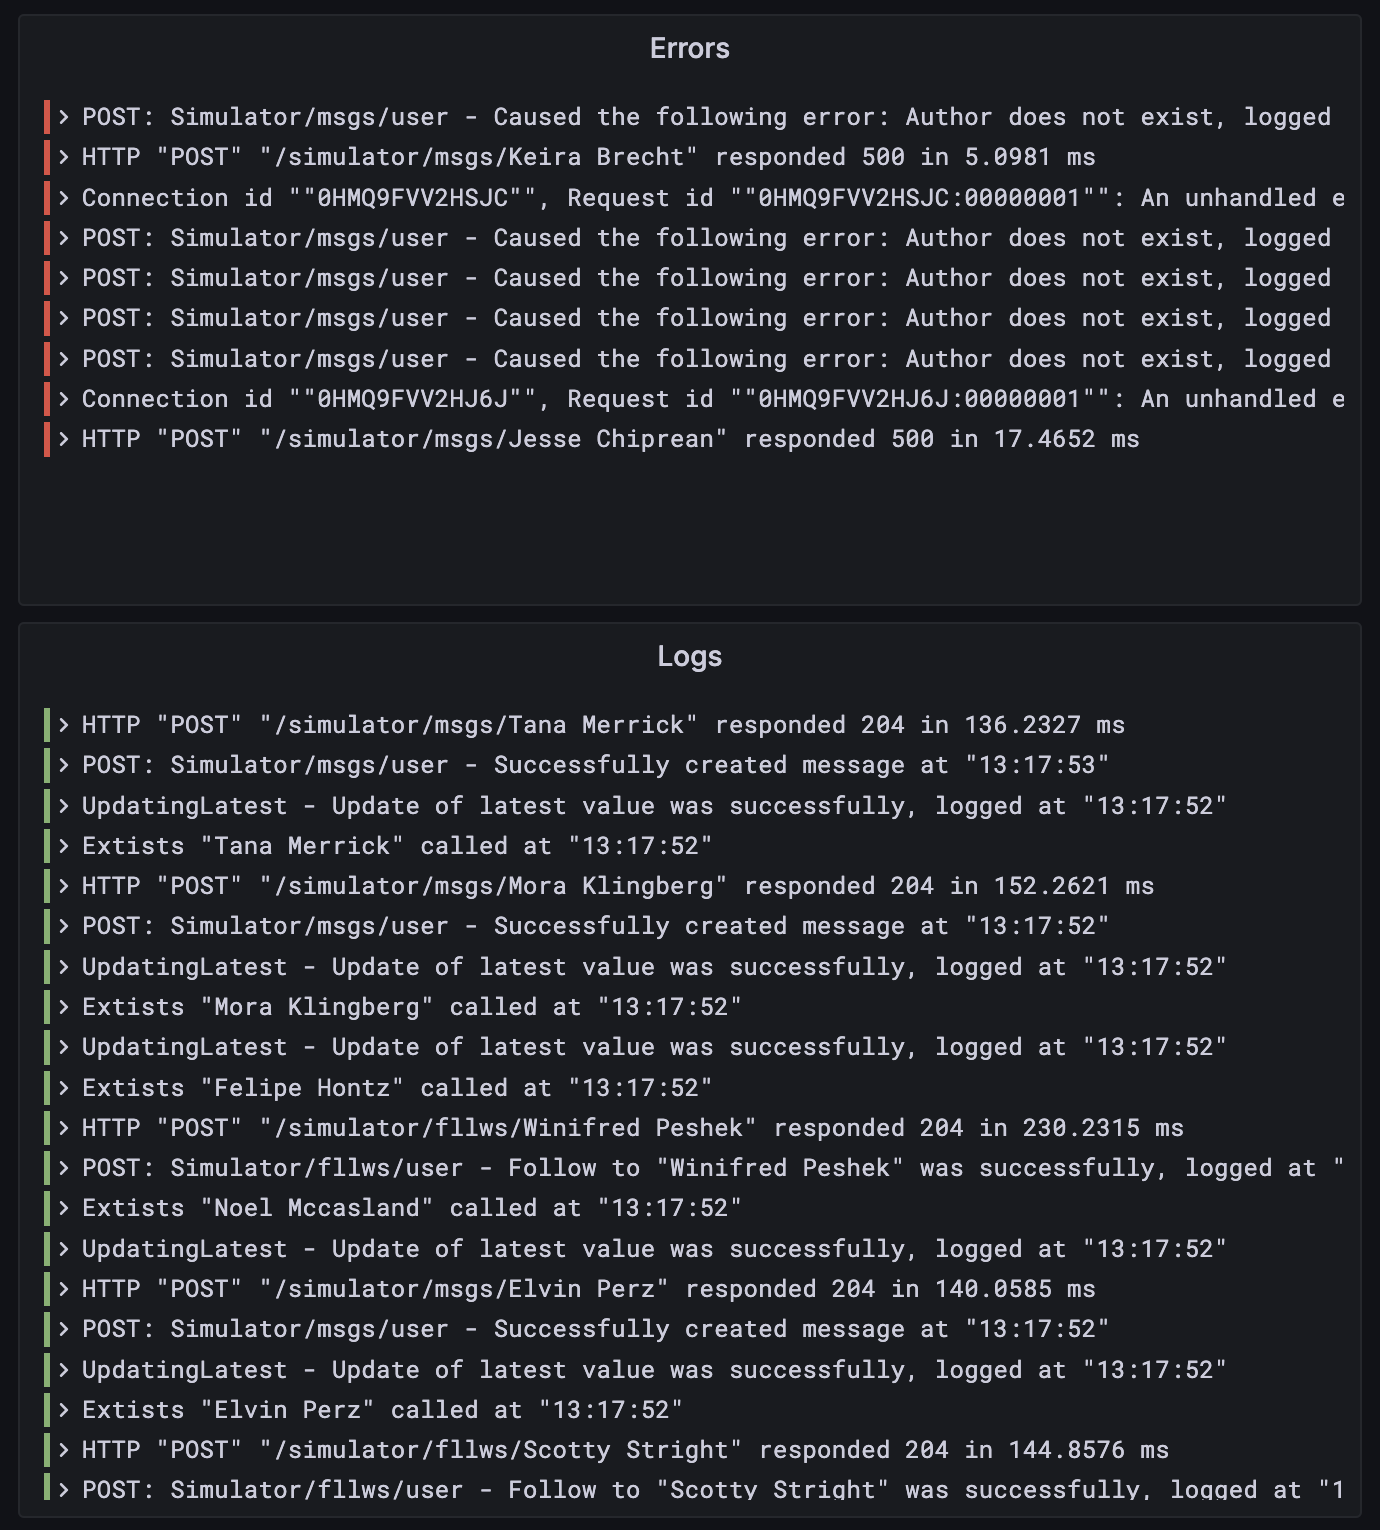
\includegraphics[width=0.45\textwidth]{images/logs_good.png} }}%
    \qquad
    \subfloat[\centering The logs when we took down the database]{{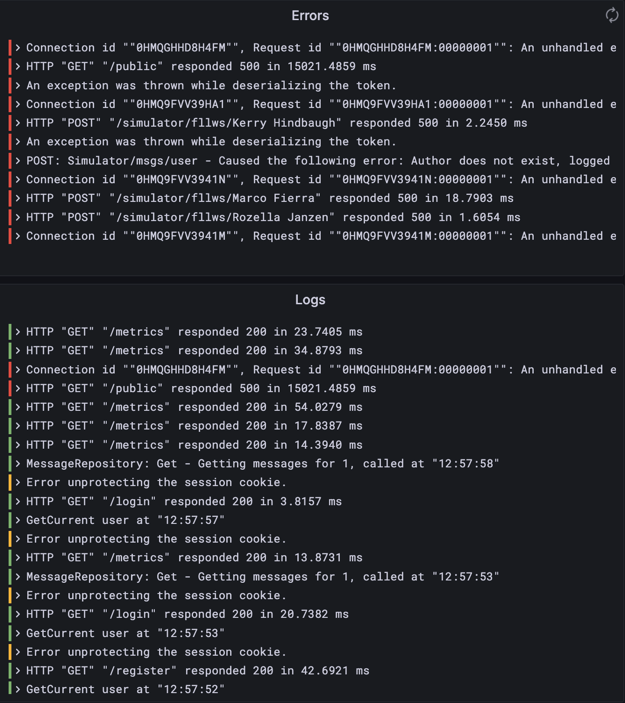
\includegraphics[width=0.45\textwidth]{images/logs_bad.png} 
    \label{fig:errors_no_db}
    }}%
    \caption{Logs.}%
    \label{fig:example}%
\end{figure}

%When we had to change the database, we first had to take it down. This is visible in our logs since we began getting a lot of errors when this was the case. This was ultimately a good sign since it meant that if something were wrong in our system, we would be able to see it immediately and fix it as fast as possible. \\

%Whenever we had downtime, new users could not be registered. However, the logs helped us with this since we had a script that could create the users from the logs directly, such that when the system was up and running again, the users who tried to register during downtown would now be registered in the database.

\subsection{Scaling And Load Balancing}
Our load balancing uses different strategies for a 'normal' user and the course simulator. When a request is made to the \textit{/simulator} endpoint, it uses the round-robin approach, which means the request is sent to any of the active servers, distributing the simulator requests across all the active servers. However, when a connection is established through the website, we are using an IP hash approach. This means that the same user is always directed to the same server, which ensures that the user session is preserved.

Scaling can be done horizontally by adding more nodes to the docker swarm. In our deployment we were using three droplets of the second lowest tier on DigitalOcean. So if scaling becomes necessary it will make more sense to start with vertical scaling by provisioning some virtual machines with more dedicated memory and processing power.
%It has not been necessary to establish a scaling strategy due to the scope of the course. Our monitoring has never indicated this to be necessary. If our current system is overloaded, it would be required to scale vertically or horizontally. Our system makes it easy to scale horizontally, the only real change being having to change our infrastructure as code scripts. Scaling vertically is easy through Digital Ocean.

\subsection{Security Assessment}
We decided to do a security assessment to discover potential security flaws in our system implementation. This was done through the following process: 
\begin{enumerate}
    \item Identifying the different components of the system.
    \item Identify which component posed potential security breaches and what these were for each component.
    \item Constructing risk scenarios on each potential security breach.
    \item Performing a risk analysis on the different scenarios.
    \item Running a preemptive pen test on our system.
\end{enumerate}

\begin{figure}[H]
    \centering
    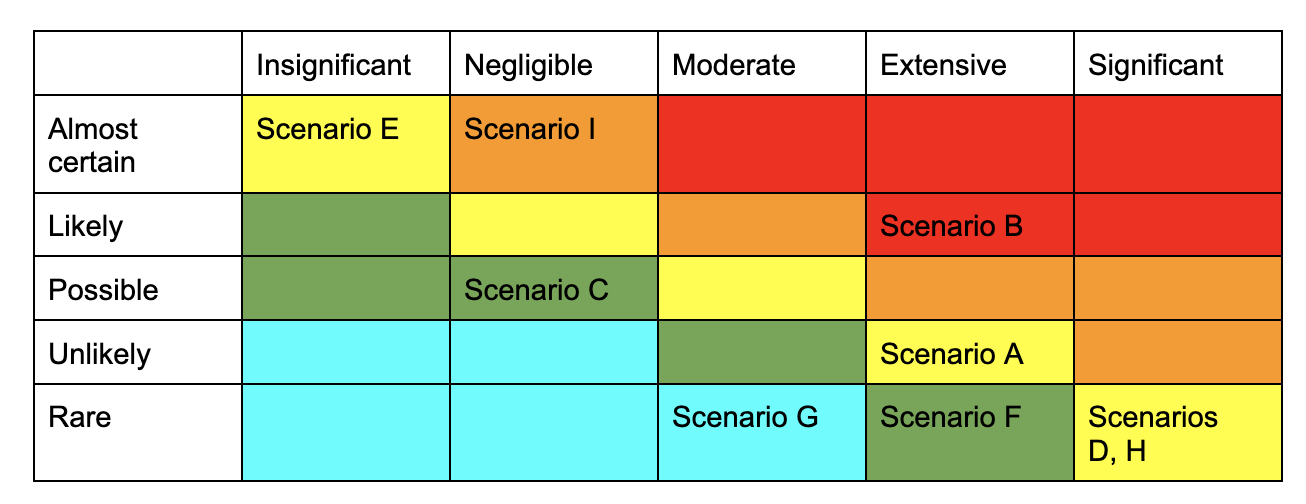
\includegraphics[width=0.8\textwidth]{images/securityAssessment.png}
    \caption{Security assessment of different risk scenarios (see appendix \ref{appendix:securityAssessment} for details on each scenario).}
    \label{fig:securityAssessmentTable}
\end{figure}

A report of our entire process can be found in appendix \ref{appendix:securityAssessment}. The security assessment matrix can be seen in figure \ref{fig:securityAssessmentTable}. The table shows us that the most critical scenario is (B) where an attacker performs a DDOS attack to make our server unresponsive. This would make our service useless and could be very bad for business. However, there is no imminent way to mitigate this other than scaling the application, having a load balancer, or paying for DDOS protection. Our system has a load balancer, but the other options were deemed to be outside this project's scope.

While the security assessment has helped us realize which parts of the system are most vulnerable and how they might be attacked, it does not guarantee that our system is not exploitable or that every possible scenario is considered. The most typical way to discover security flaws is when an attacker takes advantage of them. The security assessment did, however, give us confidence that the most ordinary tools for discovering weaknesses didn't find anything on our system. 

We have also used Snyk for checking vulnerabilities in the system. Based on our findings, changing any parts of the system was unnecessary.

\subsection{AI assistants}
In this project, we used ChatGPT. It did not write any of our source code, but it was helpful for error handling. When googling an error, finding the correct stack overflow response can sometimes be difficult, whereas, with ChatGPT, we could paste the error message, and it could often point us in the right direction. It has also been useful for setting up Nginx and docker swarm. For instance, ChatGPT provided help on how to use IP hash for keeping sessions while using load balancers.

%We tried not to rely on it too much to keep the work as authentic as possible. While getting help from it can be helpful, we never copy/pasted anything it gave us. Instead, we used ChatGPT as an extra TA.